\documentclass[hyperref={pdfpagelabels=false}]{beamer}
\usepackage{ragged2e}
\renewcommand{\raggedright}{\leftskip=0pt \rightskip=0pt plus 0cm}
\usepackage{lmodern}
\usepackage{fontspec}
\usepackage{xeCJK}
\setCJKmainfont{Noto Sans CJK TC}   % Overleaf 可用的楷體
\usepackage[english]{babel}
\usepackage{amsmath,amssymb,amsfonts,amsthm}
\hypersetup{colorlinks=true, citecolor=blue, urlcolor=blue, pdfborder={0 0 0}}
\usepackage{listings}
\usepackage{accsupp}
\newcommand{\emptyaccsupp}[1]{\BeginAccSupp{ActualText={}}#1\EndAccSupp{}}
\usepackage{tikz}
\usetikzlibrary{arrows,decorations.pathmorphing,backgrounds,fit,positioning,shapes.symbols,chains}
\newcommand{\indep}{\perp\!\!\!\perp}
\newcommand{\nindep}{\not\!\perp\!\!\!\perp}
\beamertemplatefootpagenumber



\title[]  
%{Introduction to Causal Inference and Big Data}
{Causal Inference and Data Science in Economics: An Introduction}

%\subtitle
%{免除部分負擔對幼兒醫療利用與健康的影響:斷點迴歸分析}

%\author 
 %{Tzu-Ting Yang\inst{1} \and Hsing-Wen Han\inst{2} \and Hsien-Ming Lien\inst{3}}

%\institute[short]{\inst{1} Academia Sinica \and \inst{2} Tamkang University \and \inst{3} National Chengchi University}


\author 
 {Prof. Tzu-Ting Yang  \\ 楊子霆}

\institute{Institute of Economics, Academia Sinica  \\ 中央研究院經濟研究所}
%\institute{Institute of Economics, Academia Sinica  \\ IMES/IDAS, NCCU}
%\author 
 %{楊子霆 \\ 中研院經濟所}

%\institute 
%{中正大學國際經濟專題研討}




\date
 {\today}

%\usetheme{Boadilla}
%\useinnertheme{rectangles}

\usepackage{beamerthemeshadow}
%\usecolortheme{seahorse}
\setbeamertemplate{footline}{%
	\hfill\usebeamercolor[fg]{page number in head/foot}%
	\usebeamerfont{page number in head/foot}%
	\insertframenumber\,/\,\inserttotalframenumber\hspace{1em}\vspace{2pt}%
}
%\usepackage{beamerthemeshadow}
\beamersetuncovermixins{\opaqueness<1>{25}}{\opaqueness<2->{15}}

\begin{document}


\begin{frame}{}
 \titlepage
\end{frame}


\begin{frame}{About Me}
	\begin{itemize} 
		\item Name: Yang, Tzu-Ting (楊子霆)
		\vspace{0.3cm}
		\item Affiliation:
					\vspace{0.3cm} 
			\begin{itemize}
		\item Institute of Economics, Academia Sinica		 
			\vspace{0.3cm}
		\item Office at Academia Sinica: 中央研究院經濟研究所B308
		\vspace{0.3cm}
			\end{itemize}
		\item Other Appointments: 
					\begin{itemize}
											\vspace{0.3cm}			
			\item NCCU-IMES, NTU-ECON, and NTU-AGEC			 
					\vspace{0.3cm}			
		\item Office at NCCU: 271204 General Purpose Building 
		
			\end{itemize}
				\vspace{0.3cm}
		\item Research Fields: Public/Labor Economics and Applied Econometrics
		\vspace{0.3cm}
		\item Website: \url{https://sites.google.com/view/cpelab/}
		\vspace{0.3cm}
		\item Email: \url{tty@g.nccu.edu.tw}
					%\begin{itemize}
		%\vspace{0.3cm}
		%\item Office Hour: Make an appointment	
		%	\end{itemize}
		%\vspace{0.3cm}
		%\item Course Website: %\url{https://causaldatalab.wordpress.com/2021/02/21/causal-inference-and-data-science-in-economics-spring-2021/}
	\end{itemize}
\end{frame}


\begin{frame}{Course Co-Instructor}
\begin{itemize} 

\item This course is co-taught with Prof. Huang Po-Chun (黃柏鈞)
\vspace{0.2cm}

\item Affiliation:
\vspace{0.2cm}
\begin{itemize}
\item Department of Economics, National Chengchi University
\end{itemize}

\vspace{0.2cm}

\item Research Fields:
\vspace{0.2cm}
\begin{itemize}
\item Labor Economics
\vspace{0.2cm}
\item Applied Econometrics
\end{itemize}

\vspace{0.2cm}
\item Office at NCCU: 270143 General Purpose Building
\vspace{0.2cm}

\item Website: \url{https://sites.google.com/site/huangpoch/home}
\vspace{0.2cm}
		\item Email: \url{huangpo5@nccu.edu.tw}
\end{itemize}
\end{frame}



\begin{frame}{This Course}
	%\begin{frame}{Economics, Causal Inference and Data Science}
	\begin{itemize} 
		
		\item The goal of this course is equip students with a comprehensive set of statistical tools that are useful in conducting high-quality empirical research in economics
		\vspace{0.2cm}
		\item Specifically, the course places a strong emphasis on \textbf{causal inference} and understanding their applications
		\vspace{0.2cm}
		\item We will especially focus on the practical implementation of these empirical methods by writing a term paper
		\vspace{0.2cm}
		\begin{itemize} 
			\item  How to conduct an empirical research
			\vspace{0.2cm}
			\item Provide a good start for your thesis
		\end{itemize}
	\end{itemize}
\end{frame}






\title[]  
{Economics, Causal Inference and Data Science}


\author 
{}

%\institute{Institute of Economics, Academia Sinica  \\ Econ, NTU}
%\institute{Institute of Economics, Academia Sinica  \\ IMES/IDAS, NCCU}
\institute{}

%\author 
%{楊子霆 \\ 中研院經濟所}

%\institute 
%{中正大學國際經濟專題研討}




\date
{}


\begin{frame}{}
	\titlepage
\end{frame}









\begin{frame}{Economics, Causal Inference and Data Science}
	%\begin{frame}{Economics, Causal Inference and Data Science}
	\begin{itemize} 
		\item Empirical research is experiencing two methodological
		``revolutions" over the past few decades
		\vspace{0.2cm}
		\item On the one hand, there is the ``credibility revolution" 
		\vspace{0.2cm}
		\begin{itemize} 
			\item A movement that emphasizes the goal of empirical research is to understand causality
					\vspace{0.2cm}
			\item Labor economists play an crucial role in this movement
		\end{itemize}
		
		
	\end{itemize}
\end{frame}



\begin{frame}{2021 Nobel Laureates}{Causal Inference in Economics}
	
%{Labor Economics and Causal Inference}
	
	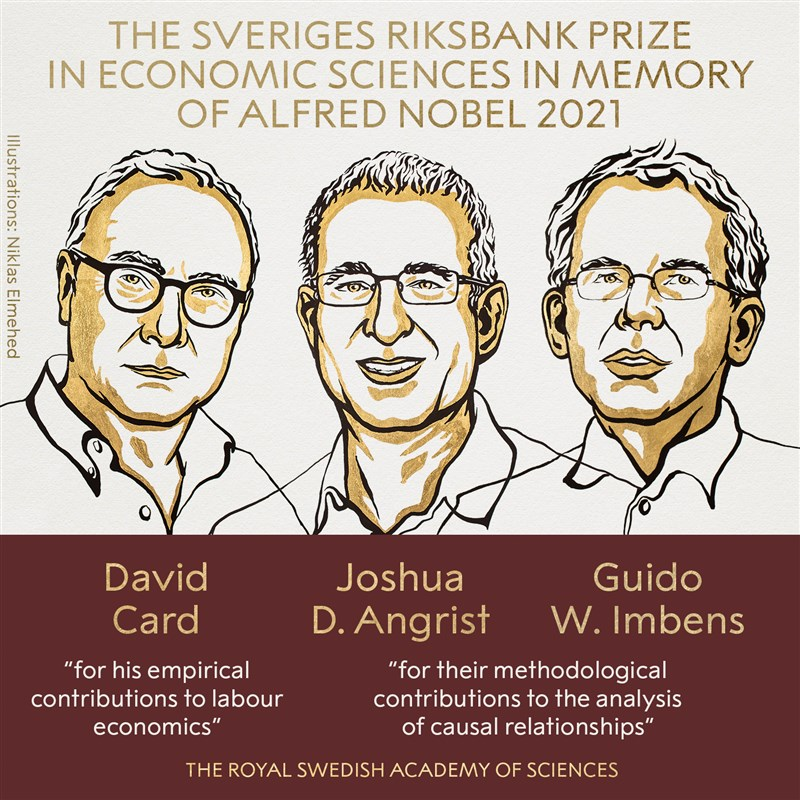
\includegraphics[width=0.65\textwidth]{figure/2021_norbel_prize.jpg}
	
\end{frame}



\begin{frame}{Economics, Causal Inference and Data Science}

\begin{itemize} 

\item On the other hand, there is the ``big data revolution"
\vspace{0.2cm} 

\begin{itemize} 
\item A movement that emphasizes how our increasing ability to collect and analyze vast amounts of data can transform our understanding of human behavior
\end{itemize}

\vspace{0.2cm} 

\item Recent trend in empirical research 
\vspace{0.2cm} 

\begin{itemize} 
\item Use large-scale datasets to identify causal relationships
\vspace{0.2cm}
\item Emerging role of generative AI in automating data processing, coding, and workflow design
\vspace{0.2cm}
\item AI-assisted tools reduce technical barriers, but do not replace identification strategy or economic reasoning
\end{itemize}	

\end{itemize}

\end{frame}




\begin{frame}{Economics, Causal Inference and Data Science}
	%\begin{frame}{Economics, Causal Inference and Data Science}
	\begin{itemize} 
		\item Economic theory plays an important role in the causal analysis of large data sets with complex structure
		\vspace{0.3cm}
		\begin{itemize} 
			\item It can be difficult to study this type of data or even to decide which variables to construct
			\vspace{0.3cm}
			\item Economic models can provide conceptual frameworks to point out what are key variables or what kind of relationship we should care about
			\vspace{0.3cm}
		\end{itemize}	
		\item Better data and more credible empirical methods can help researchers test economic theories that had previously been difficult to assess
		
		
		
	\end{itemize}
\end{frame}



\begin{frame}{This course}
	%\begin{frame}{Economics, Causal Inference and Data Science}
	\begin{itemize} 
		
		\item This course will go through several useful techniques based on recent methodological developments in empirical methods  
		\vspace{0.2cm}
		\begin{itemize} 
			\item Focus on \textbf{causal inference} and its applications in economics 
			%\vspace{0.2cm}
			%\item How to conduct an empirical research
		\end{itemize}
	\end{itemize}
\end{frame}




\title[]  
{Causal Inference}


\author 
{}

%\institute{Institute of Economics, Academia Sinica  \\ Econ, NTU}
%\institute{Institute of Economics, Academia Sinica  \\ IMES/IDAS, NCCU}
\institute{}

%\author 
%{楊子霆 \\ 中研院經濟所}

%\institute 
%{中正大學國際經濟專題研討}




\date
{}


\begin{frame}{}
	\titlepage
\end{frame}


\begin{frame}{Causal Inference}
	\begin{itemize} 
		\item Social science (Economics) theories are almost always causal in their nature
		\begin{itemize} 
			\vspace{0.2cm}
			\item X causes Y
			\vspace{0.2cm}
			\item An increase in price of oil causes consumer's demand for oil to decrease
			\vspace{0.2cm}
			\item An increase in schooling years can raise people's productivity (wage)
			\vspace{0.2cm}
			\item Raising minimum wage would reduce employment opportunity of low-skilled workers
		\end{itemize}
		
	\end{itemize}
	
\end{frame}




\begin{frame}{Causal Inference}
	\begin{itemize} 
		
		\item Two key features of causality:
		\begin{itemize} 
			\vspace{0.2cm}
			\item[1] Causes are asymmetrical 
			\vspace{0.2cm}
			\begin{itemize}
				\item In general, if X causes Y, Y does not cause X
			\end{itemize}
			\vspace{0.2cm}
			\item[2] Causes are effective
			\vspace{0.2cm}
			\begin{itemize} 
				\item  A cause must be distinguished from an accidental correlation %and must bring about its effect
			\end{itemize}
		\end{itemize}
	\end{itemize}
\end{frame}


\begin{frame}{Correlation is not Causality}{Chocolate Consumption and Nobel Laureates}
	
	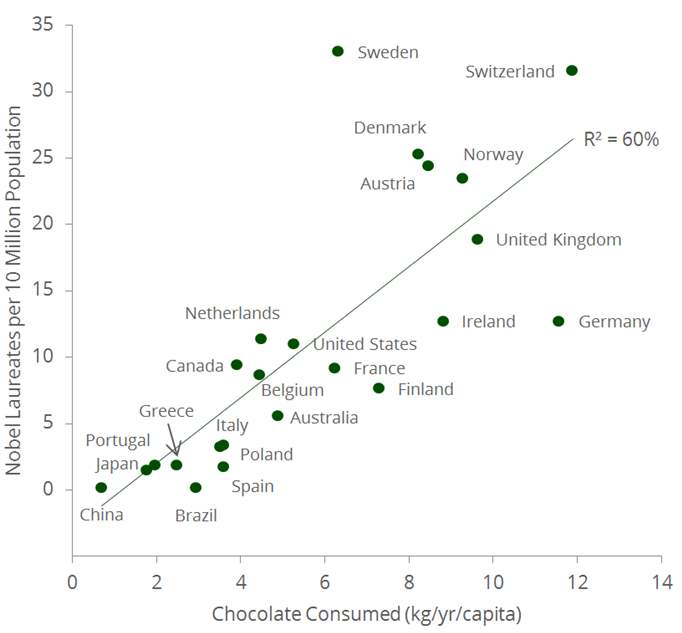
\includegraphics[width=0.65\textwidth]{figure/corr_causal.png}
	
\end{frame}


%\begin{frame}{Correlation is not Causality}{Chocolate Consumption and Nobel Laureates}

%	
\includegraphics[width=0.75\textwidth]{corr_causal_pic.png}

%\end{frame}



\begin{frame}{Correlation is not Causality}
	
	
	\begin{itemize}
		
		\item In order to increase number of Nobel Laureates (proxy for human capital)
		\vspace{0.2cm}
		\item Should government enforce everyone to eat chocolate everyday?
		
		
		
	\end{itemize}
\end{frame}





\begin{frame}{Correlation is not Causality}
	\begin{figure}
		\begin{tikzpicture}[comment/.style={rectangle, text centered}]
		\centering
		\node (u) {$U$};
		\node (X) [below=0.5 of u, xshift=-1.5em] {$X$};
		%\node (Z) [left =1.5em of D] {$Z$};
		\node (Y) [below=0.5 of u, xshift=1.5em] {$Y$};
		
		\draw [->] (u) -- node [auto]{}  (X);
		\draw [->] (u) -- node [auto]{}  (Y);
		%\draw [->] (D) -- node [auto]{}  (Y);
		%\draw [->] (Z) -- node [auto]{}  (D);
		%\draw[<->, >=latex', shorten >=2pt, shorten <=2pt, bend right=30, thick, color=red] 
		%(Z.south) to node[auto, swap] {exclusion restriction}(Y.south);
		%\node  [comment, below = 0.08 of D] (1) {\Large\color{red}$\times$};
		\end{tikzpicture}
	\end{figure}
	
	
	\begin{itemize}
		\item $X$ (Chocolate Consumption) is associated (correlated) with $Y$ (Number of Nobel Laureates) 
		\vspace{0.2cm}
		\item Even if $X$ has no causal effect on $Y$
		\vspace{0.2cm}
		\item Since confounding factor $U$ (GDP) can result in the co-movement between $X$ and $Y$
		
		
		
	\end{itemize}
\end{frame}





\begin{frame}{Causal Inference}
	\begin{itemize} 
		
		\item Understanding a causal relationship is useful for making predictions about the consequences of changing circumstances or policies
		\vspace{0.3cm}
		\item Causal inference is a type of statistical methods that help us verify the causal relationship
		\vspace{0.3cm}
		\item In general, a typical causal question is:
		\begin{itemize} 
			\vspace{0.3cm}
			\item The effect of a \color{blue}{treatment} \color{black}{on} an \color{red}{outcome}
			\vspace{0.3cm}
			\item \color{red}{Outcome}: \color{black}{A variable that we are interested in}
			\vspace{0.3cm}
			\item \color{blue}{Treatment}: \color{black}{A variable that has the (causal) effect on our outcome of interest}
			
		\end{itemize}
	\end{itemize}
\end{frame}


\begin{frame}{Causal Inference}{Example 1}
	\begin{itemize} 
		
		\item The effect of \color{blue}{getting a master's degree} \color{black}{on} \color{red}{earnings}
		\vspace{0.2cm}
		\begin{itemize}
			%\item What is the causal effect of \textbf{getting a master's degree} v.s. \textbf{not getting a master's degree} on worker's earnings
			%\vspace{0.2cm}
			\item Ideally, we should get causal effect by comparing the earnings of \textbf{the same individuals} with and without receiving a master's degree
			\vspace{0.2cm}
			\item For each particular individual, we can observe \textbf{only one outcome with specific treatment at the same time}: 
			\vspace{0.2cm}
			\begin{itemize}
				\item Getting a master's degree
				\vspace{0.2cm}
				\item Not getting a master's degree
			\end{itemize}
			
			\vspace{0.2cm}
			\item  The \textbf{unobserved outcome} is called the ``\textbf{counterfactual}" outcome
			
		\end{itemize}
		
		
		
	\end{itemize}
\end{frame}



\begin{frame}{Causal Inference}{Example 1}
	\begin{itemize} 
		
		
		\item The effect of \color{blue}{getting a master's degree} \color{black}{on} \color{red}{earnings}
		\vspace{0.2cm}
		\begin{itemize}
			\item What if we compare observed outcomes: 
			\vspace{0.2cm}
			\begin{itemize}
				\item Earnings of those getting a master's degree
				\vspace{0.2cm}
				\item Earnings of those choosing not to get it 
				\vspace{0.2cm}
			\end{itemize}
			\item Simply comparing those who are and are not treated may provide a misleading estimate of a causal effect    
			\vspace{0.2cm}
			\item There must be a reason why some people choose to have and some choose to not have a master's degree  
			\vspace{0.2cm}
			\begin{itemize}
				\item For example, those who get a master's degree may be from rich families or have high ability
				\vspace{0.2cm}
				\item Two groups of people might not be comparable
			\end{itemize}
			\vspace{0.2cm}
			\item We need to isolate casual effect from the effect of other confounding factors
		\end{itemize}
		
		
		
	\end{itemize}
\end{frame}







\begin{frame}{Causal Inference}{Example 2}
	\begin{itemize} 
		\item Macro economists also ask casual questions !
		\vspace{0.2cm}
		\item The effect of \color{blue}{fiscal stimulus spending} \color{black}{on} \color{red}{economic growth}
\vspace{0.3cm}

\begin{itemize}
\item Does government stimulus increase GDP growth?
\vspace{0.2cm}
\item Ideally, we want to compare the \textbf{same country} with and without stimulus
\vspace{0.2cm}
\item But we cannot observe both outcomes
\end{itemize}

\end{itemize}
\end{frame}



\begin{frame}{Causal Inference}{Example 2}
\begin{itemize}

\item Compare countries with stimulus vs. without stimulus?
\vspace{0.3cm}

\begin{itemize}
\item Governments often implement stimulus during recessions
\vspace{0.2cm}
\item Countries with weak growth are more likely to adopt stimulus
\vspace{0.2cm}
\item $\Rightarrow$ Simple comparison may underestimate the true effect
\end{itemize}

\end{itemize}
\end{frame}



\begin{frame}{Causal Inference}{More Examples}
\begin{itemize} 
\item More examples include:
\vspace{0.3cm}

\begin{itemize} 

\item The effect of advertisement on product sales
\vspace{0.2cm}

\item The effect of military service on earnings and employment
\vspace{0.2cm}

\item The effect of unemployment insurance on job search behavior
\vspace{0.2cm}

\item The effect of credit regulation on housing prices
\vspace{0.2cm}

\item Do immigrant workers depress the wages of native workers?
\vspace{0.2cm}

\item Does eliminating estate tax increase wealth inequality?
\vspace{0.2cm}

\item Can democracy increase economic growth?
\vspace{0.2cm}

\item What is the effect of \textbf{AI adoption} on firm productivity?
\vspace{0.2cm}

\item Does the introduction of \textbf{generative AI tools} change worker wages or employment?
\vspace{0.2cm}

\item What is the long-term impact of COVID-19 on the global economy?

\end{itemize}

\end{itemize}
\end{frame}


\begin{frame}{Causal Inference}
	\begin{itemize} 
		\item The fundamental problem of inferring the causal effect is that:
		\vspace{0.2cm}
		\begin{itemize}
			\item For every unit (e.g. individual, household, state, or country), we fail to observe the outcome if the chosen level of the treatment had been different
		\end{itemize}
		\vspace{0.3cm}
		\item Basically, causal inference is the study of \textbf{unobservable counterfactuals}:
		\begin{itemize} 
			\vspace{0.3cm}
			\item It tells us what happend in alternative (or ``counterfactual") world
			\vspace{0.3cm}
			\item What would happened if we were to change this aspect of the world ?
		\end{itemize}
		
		
		
		
	\end{itemize}
\end{frame}



\begin{frame}{Causal Inference}{Unobservable Counterfactuals}
	
	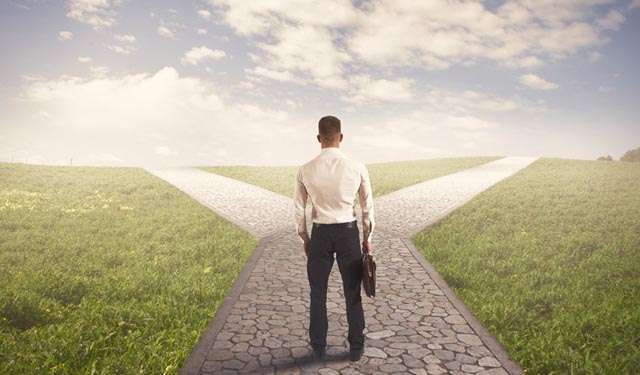
\includegraphics[width=1.0\textwidth]{figure/two_way.jpg}
	
\end{frame}



\begin{frame}{Causal Inference}
	\begin{itemize} 
		
		\item Since it is impossible to observe the \textbf{unobserved} counterfactual outcome
		\vspace{0.3cm}
		\item Causal inferences help us infer the values of these \textbf{unobserved counterfactual outcomes} from \textbf{observed data} by imposing specific assumptions
		\vspace{0.3cm}
		%\item Under specific assumptions, we can infer the values of these unobserved counterfactual outcomes from observed data	
		%		\vspace{0.3cm}
		\item Under specific assumptions, we are able to construct a comparison group that can represent counterfactual outcomes
				\vspace{0.3cm}
		\item Then, we can obtain the causal effect of treatment
		

		
		%say the observed control group is comparable to treatment group		
		
		%\item Assumption-free causal inference is impossible!		
		
		
	\end{itemize}
\end{frame}






\title[]  
{Course Content: Causal Inference}


\author 
{}

%\institute{Institute of Economics, Academia Sinica  \\ Econ, NTU}
%\institute{Institute of Economics, Academia Sinica  \\ IMES/IDAS, NCCU}
\institute{}

%\author 
%{楊子霆 \\ 中研院經濟所}

%\institute 
%{中正大學國際經濟專題研討}




\date
{}


\begin{frame}{}
	\titlepage
\end{frame}




\begin{frame}{Course Content: Randomized Experiment}{Prof. Tzu-Ting Yang}
\begin{itemize}

\item Randomized experiment (RCT) is a gold standard of causal inference

\vspace{0.2cm}

\item Random assignment ensures:
\vspace{0.2cm}

\begin{itemize}
\item Treatment assignment is unrelated to observed and unobserved confounders
\vspace{0.2cm}
\item This feature will make treatment and control groups statistically comparable
\end{itemize}

\vspace{0.2cm}

% \item Causal effect = simple difference in average outcomes

% \vspace{0.2cm}

\item Limitations
\vspace{0.2cm}

\begin{itemize}
\item Often costly, unethical, or infeasible
\vspace{0.2cm}

\item Many important economic questions cannot be randomized
\end{itemize}

\vspace{0.2cm}

\item In this course:
\vspace{0.2cm}

\begin{itemize}
\item We briefly introduce RCT logic
\vspace{0.2cm}

\item Main focus: the methods when we can not implement RCT 
\end{itemize}

\end{itemize}
\end{frame}




\begin{frame}{Course Content: Model-Based Methods}{Prof. Tzu-Ting Yang}
\begin{itemize}

\item[1.] Matching Methods
\vspace{0.2cm}

\begin{itemize}
\item Assume selection is based on observables
\vspace{0.2cm}
\item Construct comparison group with similar observable characteristics
\end{itemize}

\vspace{0.2cm}

\item[2.] Regression and Causal Machine Learning
\vspace{0.2cm}

\begin{itemize}
\item Control for observable confounders using regression
\vspace{0.2cm}
\item Use ML tools (e.g., Post-Double Selection) for variable selection
\end{itemize}

\vspace{0.2cm}

\item[3.] Fixed Effect Regression
\vspace{0.2cm}

\begin{itemize}
\item Control for time-invariant unobserved heterogeneity
\vspace{0.2cm}
\item Common in panel data settings (individual, firm, region FE)
\end{itemize}

\end{itemize}
\end{frame}



\begin{frame}{Course Content: Design-Based Methods}{Prof. Po-Chun Huang}
\begin{itemize}

\item[4.] Differences-in-Differences (DID)
\vspace{0.2cm}

\begin{itemize}
\item Requires parallel trends assumption
\vspace{0.2cm}

\item Use untreated group's trend as counterfactual
\end{itemize}

\vspace{0.2cm}

\item[5.] Synthetic Control Method (SCM)
\vspace{0.2cm}

\begin{itemize}
\item Data-driven weighted combination of control units
\vspace{0.2cm}

\item Suitable when parallel trends do not hold
\end{itemize}



\end{itemize}
\end{frame}




\begin{frame}{Course Content: Design-Based Methods}{Prof. Po-Chun Huang}
\begin{itemize}

\item[6.] Regression Discontinuity Design (RDD)
\vspace{0.2cm}

\begin{itemize}
\item Treatment assigned by cutoff rule
\vspace{0.2cm}

\item Compare observations just above and below threshold
\end{itemize}

\vspace{0.2cm}

\item[7.] Instrumental Variables (IV)
\vspace{0.2cm}

\begin{itemize}
\item Use exogenous variation that affects treatment
\vspace{0.2cm}

\item Exclusion restriction: instrument affects outcome only via treatment
\end{itemize}

\end{itemize}
\end{frame}


\begin{frame}{Course Content: Advanced Topics}{Prof. Tzu-Ting Yang}
	\begin{itemize} 
		
		\item[8.] Shift-Share IV Design
	\vspace{0.3cm}
		\begin{itemize} 
	\item  Utilizes an instrument based on national trends in the treatment exposure that are unrelated to local confounders
		\end{itemize}
		\vspace{0.3cm}
		\item[9.] Spatial RD Design
		\vspace{0.3cm}	
		\begin{itemize} 
			\item Estimate treatment effects by comparing observations just above and below a geographic boundaries for treatment assignment		
		\end{itemize}
		\vspace{0.3cm}	
		\item[10.] Causal Forest
		\vspace{0.3cm}	
		\begin{itemize} 
			\item A machine learning technique used to estimate heterogeneous treatment effects
		\end{itemize}

		
	\end{itemize}
\end{frame}







\title[]  
{Course Content: Data Analysis}


\author 
{}

%\institute{Institute of Economics, Academia Sinica  \\ Econ, NTU}
%\institute{Institute of Economics, Academia Sinica  \\ IMES/IDAS, NCCU}
\institute{}

%\author 
%{楊子霆 \\ 中研院經濟所}

%\institute 
%{中正大學國際經濟專題研討}




\date
{}


\begin{frame}{}
	\titlepage
\end{frame}



\begin{frame}{Data Analysis and Research Workflow}{}
\begin{itemize}

\item Credible causal inference requires a well-constructed dataset
\vspace{0.2cm}

\item Creating an ``analysis-ready'' dataset is often the most time-consuming step
\vspace{0.2cm}

\begin{itemize}
\item Data cleaning, merging, reshaping, and validation
\vspace{0.2cm}
\item Often accounts for 70--80\% of research time
\end{itemize}

\vspace{0.2cm}

\item In this course, you will do:
\vspace{0.2cm}

\begin{itemize}
\item Data cleaning and transformation
\vspace{0.2cm}
\item Constructing research variables
\vspace{0.2cm}
\item Visualization and exploratory analysis
\end{itemize}

\end{itemize}
\end{frame}


\begin{frame}{The Changing Nature of Economic Data}{}
\begin{itemize}

\item Traditional sources
\vspace{0.2cm}

\begin{itemize}
\item Government surveys
\vspace{0.2cm}
\item Official statistics
\end{itemize}

\vspace{0.2cm}

\item Data revolution in the past decade
\vspace{0.2cm}

\begin{itemize}
\item Large-scale administrative data
\vspace{0.2cm}
\item Near-universal population coverage
\end{itemize}

\vspace{0.2cm}

\item Examples in Taiwan
\vspace{0.2cm}

\begin{itemize}
\item Health insurance claims
\vspace{0.2cm}
\item Tax return data
\vspace{0.2cm}
\item Housing transaction records
\end{itemize}

\end{itemize}
\end{frame}



\begin{frame}{Unstructured and High-Dimensional Data}{}
\begin{itemize}

\item Increasing use of non-traditional data formats
\vspace{0.2cm}

\begin{itemize}
\item Text documents
\vspace{0.2cm}
\item Social media
\vspace{0.2cm}
\item Geolocation data
\vspace{0.2cm}
\item Satellite and image data
\end{itemize}

\vspace{0.2cm}

% \item Handling these datasets requires
% \vspace{0.2cm}

% \begin{itemize}
% \item Data engineering skills
% \vspace{0.2cm}
% \item Automated workflows
% \vspace{0.2cm}
% \item Reproducible coding practices
% \end{itemize}

\end{itemize}
\end{frame}





\begin{frame}{Geographic data}
	\begin{center}
		\begin{figure}[p]
			\centering
			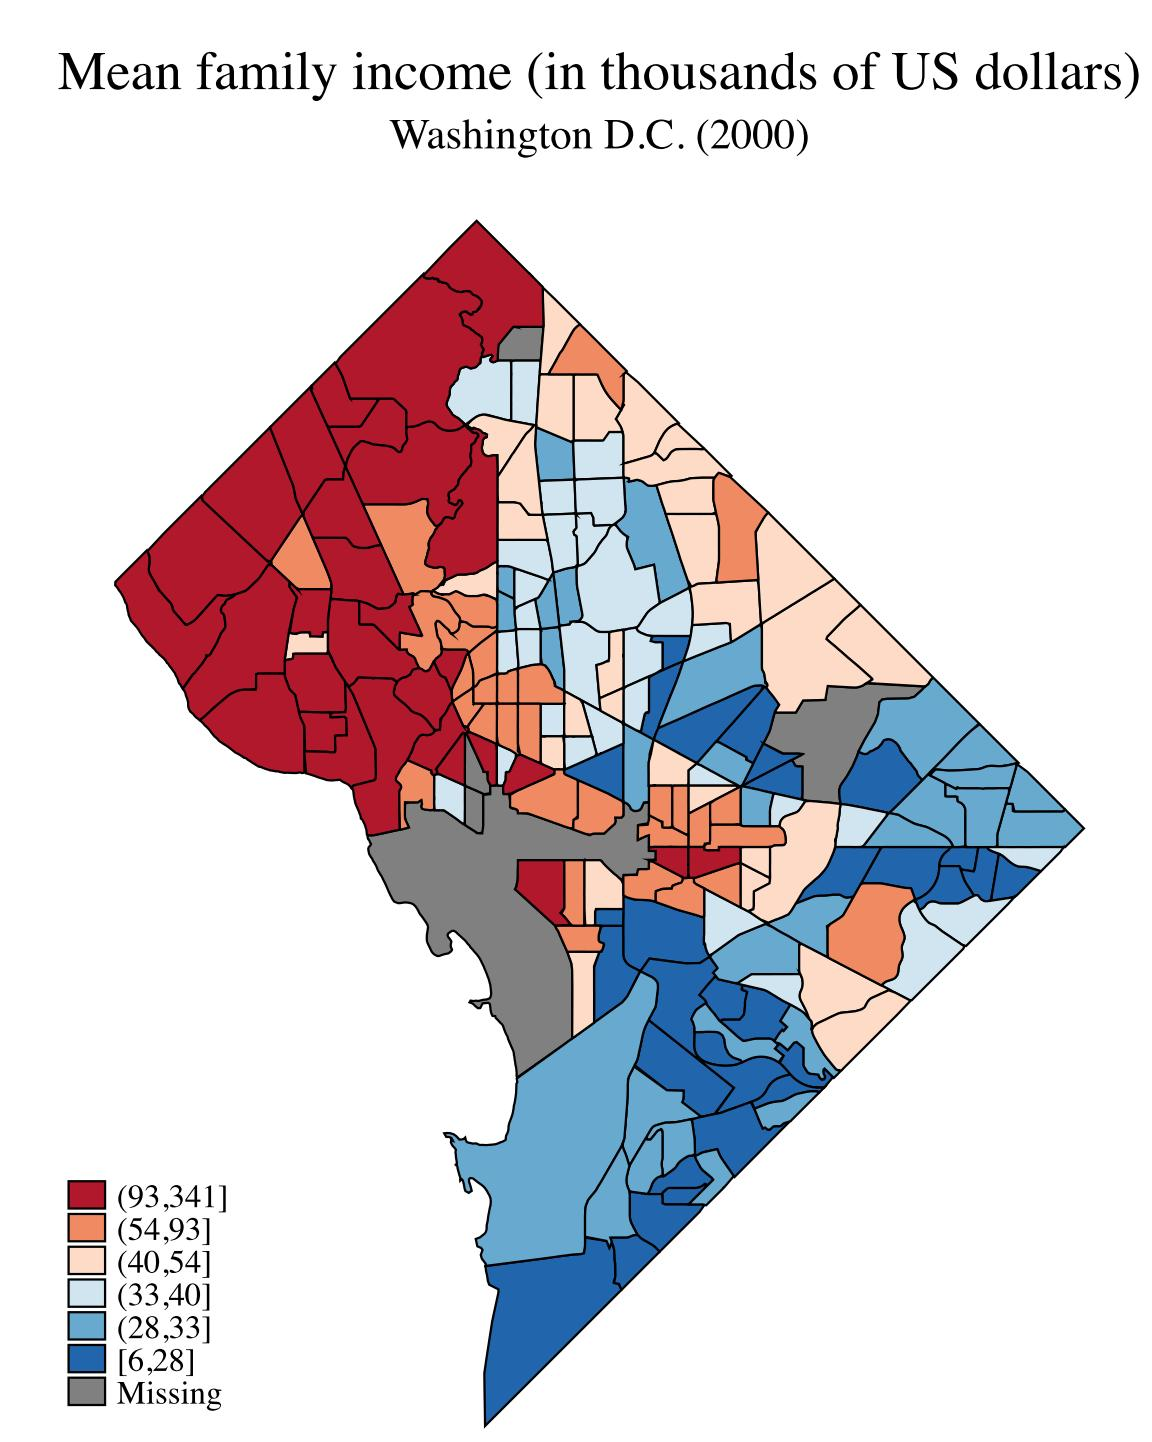
\includegraphics{figure/geo_data.jpg}
		\end{figure}
		\begin{minipage}{1.0\linewidth}
			\fontsize{8}{8pt}\selectfont
			\emph{Source:}  Maurizio Pisati (2012)
		\end{minipage}
	\end{center}
\end{frame}



\begin{frame}{Generative AI in Data Processing}{}
\begin{itemize}

\item Generative AI as a research assistant for data work
\vspace{0.2cm}

% \item Applications in empirical research
% \vspace{0.2cm}

\begin{itemize}
\item Code generation and debugging
\vspace{0.2cm}
\item Data cleaning scripts
\vspace{0.2cm}
\item Rapid prototyping ("vibe coding")
\end{itemize}

\vspace{0.2cm}

\item AI agents (e.g., Claude, Google AI tools)
\vspace{0.2cm}

\begin{itemize}
%\item Large-scale codebase navigation
%\vspace{0.2cm}
\item Automating repetitive data tasks
\vspace{0.2cm}
\item Structuring messy raw data
\end{itemize}

\vspace{0.2cm}

% \item Emphasis in this course
% \vspace{0.2cm}

% \begin{itemize}
% \item Responsible use of AI tools
% \vspace{0.2cm}
% \item Verification of outputs
% \vspace{0.2cm}
% \item Reproducibility and research integrity
% \end{itemize}

\end{itemize}
\end{frame}




% \begin{frame}{Text Analysis}{}

% \begin{itemize}

% \item Rapid growth in text-based economic data
% \vspace{0.2cm}

% % \begin{itemize}
% % \item Policy documents
% % \vspace{0.2cm}
% % \item Earnings call transcripts
% % \vspace{0.2cm}
% % \item News articles and regulatory filings
% % \vspace{0.2cm}
% % \item Social media and online discussions
% % \end{itemize}

% % \vspace{0.3cm}

% \item How can LLMs help?
% \vspace{0.2cm}

% \begin{itemize}
% \item Automatically classify text into economic categories
% \vspace{0.2cm}
% \item Extract structured variables from unstructured documents
% \vspace{0.2cm}
% \item Measure tone, sentiment, and policy uncertainty
% \vspace{0.2cm}
% \item Summarize large volumes of text efficiently
% \end{itemize}

% \vspace{0.3cm}

% \item Key idea:
% \vspace{0.2cm}

% \begin{itemize}
% \item LLMs improve efficiency in text coding
% \vspace{0.2cm}
% \item Economic reasoning and identification remain the researcher's responsibility
% \end{itemize}

% \end{itemize}

% \end{frame}



% \begin{frame}{Traditional Workflow vs AI-Assisted Workflow}{Prof. Tzu-Ting Yang}

% \begin{columns}[T]

% %---------------- LEFT COLUMN ----------------
% \column{0.48\textwidth}
% \textbf{Traditional Research Workflow}
% \vspace{0.3cm}

% \begin{itemize}

% \item Data collection
% \vspace{0.2cm}

% \item Manual cleaning and reshaping
% \vspace{0.2cm}

% \item Write code from scratch
% \vspace{0.2cm}

% \item Debug through trial and error
% \vspace{0.2cm}

% \item Documentation after coding
% \vspace{0.2cm}

% \item Slow iteration cycle

% \end{itemize}


% %---------------- RIGHT COLUMN ----------------
% \column{0.48\textwidth}
% \textbf{AI-Assisted Research Workflow}
% \vspace{0.3cm}

% \begin{itemize}

% \item Data collection + AI-assisted structuring
% \vspace{0.2cm}

% \item Automated cleaning script generation
% \vspace{0.2cm}

% \item Rapid prototyping ("vibe coding")
% \vspace{0.2cm}

% \item AI-supported debugging and refactoring
% \vspace{0.2cm}

% \item Auto-generated documentation
% \vspace{0.2cm}

% \item Faster iteration and experimentation

% \end{itemize}

% \end{columns}

% \vspace{0.4cm}

% \textbf{Key Message:} AI changes the speed and scale of data work, but identification and verification remain the researcher’s responsibility.

% \end{frame}


% \begin{frame}{Data Analysis}
% 	\begin{itemize} 
% 		\item A good causal inference requires a well-established DATA
% 		\vspace{0.3cm}
% 		\item Create an ``analysis-ready" dataset is a challenging task, especially for large-scale data or unstructured data
% 		\vspace{0.3cm}
% 		\item A lot of data analysis time is spent data cleaning and preparing data, up to 80\% of the time. 	
% 		\vspace{0.3cm}
% 		\item In this course, you will learn how to clean data, create your own dataset and visualize your data
% 		\vspace{0.3cm}
% 		\begin{itemize} 
% 			%\item Machine learning can help us create/transform data for analysis and also do preliminary analysis
% 			%\vspace{0.3cm}
% 			\item You might also learn how to collect your own data
% 		\end{itemize}
		
		
		
% 	\end{itemize}
% \end{frame}




% \begin{frame}{Data Analysis}
% 	\begin{itemize} 
% 		\item Economists had a long tradition of utilizing the evidence from data to verify their theories 
% 		\vspace{0.3cm}
% 		\item In the past, the major data sources were the government surveys
% 		\vspace{0.3cm}
% 		\item The data revolution of the past decade have a further and profound effect on economic research 
		
		
		
		
		
% 	\end{itemize}
% \end{frame}




% \begin{frame}{Data Analysis}
% 	\begin{itemize} 
		
% 		\item Increasingly, economists make use of newly available large-scale administrative data with near-universal population coverage
% 		\vspace{0.3cm}
% 		\begin{itemize}
% 			\item Health insurance claims data: 
% 			\vspace{0.3cm}
% 			\begin{itemize}
% 				\item Record every Taiwanese's healthcare utilization whenever they visit doctors
% 				\vspace{0.3cm}
% 			\end{itemize}
% 			\item Tax return data: 
% 			\vspace{0.3cm}
% 			\begin{itemize}
% 				\item Record income and wealth of each taxpayer
% 			\end{itemize}
% 						\vspace{0.3cm}
% 			\item Housing transactions Data:
% 		\vspace{0.3cm}
% 		\begin{itemize}
% 			\item Record all housing and land transactions in Taiwan
% 		\end{itemize}
			
% 		\end{itemize}
		
		
% 	\end{itemize}
% \end{frame}




% \begin{frame}{Data Analysis}
% 	\begin{itemize} 
		
		
% 		\item Due to the growth of the internet, economists also begin to use new data formats (unstructured data)
% 		\vspace{0.3cm}
% 		\begin{itemize}
% 			\item Online document
% 			\vspace{0.3cm}
% 			\item Social media
% 			\vspace{0.3cm}
% 			\item Geolocations
% 		\end{itemize}
% 		\vspace{0.3cm}
% 		\item In this course, I will also teach you how to handle with these new types of datasets 
% 		\vspace{0.3cm}
% 		\begin{itemize}
% 			\item Geographic data
% 			%\vspace{0.3cm}
% 			%\item Text data
			
% 		\end{itemize}
		
		
		
% 	\end{itemize}
% \end{frame}






\begin{frame}{Course Structure}
\begin{itemize} 

\item[1] Focus on how to implement various empirical methods of drawing causal inference
\vspace{0.3cm}

\item[2] Discuss the applications in economics
\vspace{0.3cm}

\item[3] Learn how to use statistical software and generative AI tools to conduct data analysis/empirical research
\vspace{0.3cm}

\begin{itemize}
\item Data cleaning and visualization
\vspace{0.2cm}
% \item Text and geographic data processing
% \vspace{0.2cm}
\item AI-assisted coding and workflow design
\end{itemize}

\end{itemize}
\end{frame}


\begin{frame}{Reading Materials}
	\begin{itemize} 
		\item Lecture slides: posted on my website
		\vspace{0.2cm}
		\item Suggested Readings:
		\begin{itemize}
						\vspace{0.2cm}
			\item \textbf{The Effect: An Introduction to Research Design and Causality} by Huntington-Klein	
			\vspace{0.2cm}
			\item \textbf{Causal Inference: The Mixtape} by Scott Cunningham
			\vspace{0.2cm}
			\begin{itemize}
				\item New textbook and cover more methods
				\vspace{0.2cm}
				\item Provide STATA and R examples
				\vspace{0.2cm}
			\end{itemize}
			\item \textbf{Econometric Methods for Program Evaluation} by Alberto Abadie and Matias D. Cattaneo
			\vspace{0.2cm}
			\begin{itemize}
				\item This is an academic paper not a textbook 
				\vspace{0.2cm}
				\item It can help you understand causal inference methods in a short time				
			\end{itemize}
			
			%\item \textbf{Labor Economics} by Pierre Cahuc, Stephane Carcillo and Andre Zylberberg (graduate level)
			%\vspace{0.2cm}
			%\item  \textbf{Labor Economics} by George Borjas (undergraduate level)
			
		\end{itemize}
		
	\end{itemize}
\end{frame}



\begin{frame}{Reading Materials}
	\begin{itemize} 
		
		\item Suggested Readings:
		\begin{itemize}
			\vspace{0.2cm}
			\item \textbf{Mastering Metrics: The Path from Cause to Effect} by Angrist and Pischke
			\vspace{0.2cm}
			\begin{itemize}
				\item Chatty, opinionated, but intuitive approach to causal inference
				\vspace{0.2cm}
			\end{itemize}
			\item \textbf{Mostly Harmless Econometrics} by Angrist and Pischke
			\vspace{0.2cm}
			\begin{itemize}
				\item More advanced
			\end{itemize}
			\vspace{0.2cm}
			\item \textbf{An Introduction to Statistical Learning with Applications in R} by Gareth James, Daniela Witten, Trevor Hastie and Robert Tibshirani
			\vspace{0.2cm}
			\begin{itemize}
				\item An introductory book for machine learning
				\vspace{0.2cm}
			\end{itemize}
		%	\item \textbf{Labor Economics} by Pierre Cahuc, Stephane Carcillo and Andre Zylberberg (graduate level)
		%	\vspace{0.2cm}
		%	\item  \textbf{Labor Economics} by George Borjas (undergraduate level)
			
		\end{itemize}
		
	\end{itemize}
\end{frame}



\begin{frame}{Reading Materials}
	\begin{itemize} 
		
		\item Suggested Readings:
		\begin{itemize}
			\vspace{0.2cm}
			\item \textbf{Korinek (2023), Generative AI for Economic Research}
\begin{itemize}
				\vspace{0.2cm}

\item JEL article on how LLMs assist economists across research tasks
\end{itemize}
				\vspace{0.2cm}

\item \textbf{Korinek (2025), AI Agents for Economic Research}
				\vspace{0.2cm}

\begin{itemize}
\item Update on AI agent frameworks and autonomous workflows
\end{itemize}

% \item \textbf{Jenner et al. (2025), Using LLMs for Narrative Analysis}
% \begin{itemize}
% \item Methodological paper on LLM-assisted qualitative text analysis
% \end{itemize}

% \item \textbf{Eloundou et al. (2025), GPTs are GPTs (arXiv)}
% \begin{itemize}
% \item Economics paper on labor market implications of LLMs
% \end{itemize}

% \item \textbf{Schmidt et al. (2025), Identifying economic narratives (arXiv)}
% \begin{itemize}
% \item Economic narrative extraction using LLMs
 \end{itemize}
		
	\end{itemize}
\end{frame}






\title[]  
{Course Requirements}


\author 
{}

%\institute{Institute of Economics, Academia Sinica  \\ Econ, NTU}
%\institute{Institute of Economics, Academia Sinica  \\ IMES/IDAS, NCCU}
\institute{}

%\author 
%{楊子霆 \\ 中研院經濟所}

%\institute 
%{中正大學國際經濟專題研討}




\date
{}


\begin{frame}{}
	\titlepage
\end{frame}






\begin{frame}{Course Goals}
	\begin{itemize} 
		\item Get a solid understanding of the empirical methods to estimate causal effect and conduct data analysis
		\vspace{0.3cm}
			\begin{itemize} 
		\item Be able to implement a good empirical research
		\vspace{0.3cm}
		\item Be able to critically evaluate empirical studies
		\vspace{0.3cm}
			\end{itemize}
		\item Be familiar with techniques and tricks of data management and visualiztion
		\begin{itemize}
			\vspace{0.3cm}
			\item Use STATA
			\vspace{0.3cm}
			\item Use R
		\end{itemize}
		\vspace{0.3cm}
		\item Have a good start of your thesis/writing sample
		
		%\item The goal of this class is for you to get a solid understanding of regression methods, of causality, and of (quasi-)experimental methods to estimate causal eects. The class should enable you to be a critical reader of empirical research, and to begin doing your own research.
		
	\end{itemize}
\end{frame}





\begin{frame}{Grading Policy}
\begin{itemize}	
		
\item Two empirical homework \& Two Oral Exams (30\%)
\vspace{0.3cm}	 
\begin{itemize}
\item Each homework is followed by an individual oral exam
\vspace{0.2cm}
\item The oral exam will assess your understanding of your own code and empirical design
\end{itemize}
\vspace{0.3cm}

\item Reading group presentation (15\%)
\vspace{0.3cm}

\item Term paper presentation (15\%)
\vspace{0.3cm}

\item Term paper (40\%): milestones throughout the semester
%\vspace{0.3cm}




%\item Extra 5 points (equivalent to 2 points in final grade) if you upload your codes and related files to \textit{GitHub} for replication.
		
\end{itemize}
\end{frame}



\begin{frame}{Course Requirements}
	\begin{itemize}	
		
		\item You should use \textbf{Latex} to type your term paper in Chinese or English
		\vspace{0.3cm}	 
		\begin{itemize}	
			\item \textbf{Latex} is a tool for typesetting professional-looking documents
			\vspace{0.3cm}
		\end{itemize}	
	% \item In addition, you are encouraged to upload your code to \textbf{GitHub} for replication (Bonus!)
	% \vspace{0.3cm}	 
	% \begin{itemize}	
	% \item \textbf{GitHub} is an online repository that store and share your source code projects 
	% 		\end{itemize}	
	% 	\vspace{0.3cm}	 
	\item You can use "homework" to practice the above "requirements"	
		
	\end{itemize}
\end{frame}







\begin{frame}{Important Dates}
	\begin{itemize} 
		% \item Compulsory Office Hour: March and May 
		% \vspace{0.3cm}
		\item Homework 1: 4/12
        		\vspace{0.2cm}
           	\begin{itemize}      
        \item Oral Exam 1: 4/23 week
        	\end{itemize}

		\vspace{0.2cm}
		\item Homework 2: 5/17 
                   	\begin{itemize}      

        		\vspace{0.2cm}
        \item Oral Exam 2: 5/28 Week
        	\end{itemize}

		\vspace{0.2cm}
		\item Reading group presentation: 5/28 and 6/4
		\vspace{0.2cm}
		%\item Research progress presentation: 11/15
		%\vspace{0.3cm}
		\item Term paper presentation: 6/11
		\vspace{0.2cm}
		\item Term paper deadline: 6/18
		%\vspace{0.3cm}
		%\item The final presentation plan depends on how many students will enroll in this course
	\end{itemize}
\end{frame}



\begin{frame}{Oral Exams}{4/23 week and 5/28 Week}
\begin{itemize}

\item Each oral exam will last about 20--30 minutes
\vspace{0.3cm}

\item You will be asked to explain:
\vspace{0.3cm}

\begin{itemize}
\item The code you wrote in your homework
\vspace{0.2cm}
\item The empirical question you want to study
\vspace{0.2cm}
\item The regression equation you plan to estimate
\vspace{0.2cm}
\item Why your empirical specification makes sense
\end{itemize}

\vspace{0.4cm}

\item The goal is to assess your understanding of:
\vspace{0.3cm}

\begin{itemize}
\item Empirical methods you learn in this courses
\vspace{0.2cm}
\item Statistical programming languages: R/Stata
%\vspace{0.2cm}
%\item Reseaech design
\end{itemize}

\end{itemize}
\end{frame}



\begin{frame}{Oral Exams}{4/23 week and 5/28 Week}
\begin{itemize}

\item After the oral exam, we will discuss your term paper progress
\vspace{0.2cm}
\begin{itemize}
\item Discuss/Refine your research question
\vspace{0.2cm}
\item Clarify identification strategy
\vspace{0.2cm}
\item Discuss possible datasets and regression specifications
\end{itemize}

\vspace{0.2cm}

\item You can prepare in advance
\vspace{0.2cm}

\begin{itemize}
\item All questions are based on your own submitted work
\vspace{0.2cm}
\item If you understand your code and empirical design clearly, the oral exam will be straightforward
\end{itemize}

\vspace{0.2cm}

\item This format reflects the rise of generative AI tools and emphasizes genuine understanding

\end{itemize}
\end{frame}




%\begin{frame}{Key paper presentation}{4/26 and 5/3}
%\begin{itemize} 


%\item Present a key paper related to your term paper in 20-30 minutes
%\vspace{0.3cm}
%\item The same topic but different empirical methods (IV, DID, or RDD) 
%\vspace{0.3cm}
%\item The different topic but similar empirical methods
%\vspace{0.3cm}
%\item Before your presentation, you should let me know your paper choice
%\end{itemize}
%\end{frame}











\begin{frame}{Reading group presentation}{5/28 and 6/4}
	\begin{itemize} 
		\item Present one of the paper that applies causal inference from reading list
		\vspace{0.3cm}
		\item Students in a group of \textbf{3-4} persons will give a presentation
		\vspace{0.3cm}
		\begin{itemize} 
			\item[1] Introduction and Background
			\vspace{0.3cm}
			\item[2] Data and Empirical strategy
			\vspace{0.3cm}
			\item[3] Results and Conclusion 
		\end{itemize}
				\vspace{0.3cm}
		\item Around 30-40 minimutes
		%\vspace{0.3cm}
		%	\item Each presenter needs to answer some questions from    
		%	\vspace{0.3cm}
		%	\item Discuss your preliminary results
	\end{itemize}
\end{frame}



\begin{frame}{Term paper presentation}{6/11}
	\begin{itemize} 
		\item Present the research progress of your term paper
		\vspace{0.3cm}
		\item 10 minutes presentation
		\vspace{0.3cm}
		\begin{itemize} 
			\item Introduce your research question
			\vspace{0.3cm}
			\item Discuss your empirical methods
			\vspace{0.3cm}
			%\item Briefly discuss related previous literature
			%\vspace{0.3cm}
			\item Describe the data you use and summary statistics of estimated sample  
			\vspace{0.3cm}
			\item Discuss your preliminary results
		\end{itemize}
	\end{itemize}
\end{frame}







\begin{frame}{Term paper deadline}{6/18}
	\begin{itemize}
		\item Feel free to discuss your term paper with me before the deadline
		%\vspace{0.3cm} 
		%\item Send your term paper to me and Prof. Huang through email

	\end{itemize}
\end{frame}




\title[]  
{Guideline for Writing a Term Paper}


\author 
{}

%\institute{Institute of Economics, Academia Sinica  \\ Econ, NTU}
%\institute{Institute of Economics, Academia Sinica  \\ IMES/IDAS, NCCU}
\institute{}

%\author 
%{楊子霆 \\ 中研院經濟所}

%\institute 
%{中正大學國際經濟專題研討}




\date
{}


\begin{frame}{}
	\titlepage
\end{frame}





\begin{frame}{Guideline for Writing a Term Paper}
\begin{itemize} 
\item You should start early; the paper is due on 6/18
\vspace{0.3cm}

\item Short paper style: less than 3,000 words 
\vspace{0.3cm}

\begin{itemize} 
\item See \textbf{Economics Letters}
\vspace{0.3cm}
\item See \textbf{AER: Insights}
\end{itemize}

\vspace{0.3cm}

\item Typed, double-spaced, using one-inch margins and 12-point font

\end{itemize}
\end{frame}



\begin{frame}{Guideline for Writing a Term Paper}
	\begin{itemize} 
		
		%\item For undergraduate students, you can write your term paper together (maximum 2 people)
		%\vspace{0.3cm}
		\item For senior graduate students, you cannot just submit your thesis as a term paper
		\vspace{0.3cm}
		\begin{itemize} 
			\item Let me know if you have any question about this issue	
			
		\end{itemize}	
	\end{itemize}
\end{frame}



\begin{frame}{Guideline for Writing a Term Paper}
	\begin{itemize} 
		
		\item Use credible causal inference methods to answer an empirical question
		\vspace{0.3cm}
		\begin{itemize} 
			\item Test economics (social science) theory
			\vspace{0.3cm}
			\item Estimate policy effect
			\vspace{0.3cm}
			\item Any interesting questions regarding to human behavior/social phenomenon
		\end{itemize}
		\vspace{0.2cm}
		\item \textbf{Don't worry if you don't find anything significant as long as your methods are credible and you have interpreted the results well}
		
	\end{itemize}
\end{frame}




\title[] 
{How to Find Research Topics} 
%{How to Conduct Empirical Research in Economics}


\author 
{}

%\institute{Institute of Economics, Academia Sinica  \\ Econ, NTU}
%\institute{Institute of Economics, Academia Sinica  \\ IMES/IDAS, NCCU}
\institute{}

%\author 
%{楊子霆 \\ 中研院經濟所}

%\institute 
%{中正大學國際經濟專題研討}




\date
{}


\begin{frame}{}
	\titlepage
\end{frame}




\begin{frame}{Approaches to Find Research Topics}
	\begin{itemize} 
		
		%\item For undergraduate students, you can write your term paper together (maximum 2 people)
		%\vspace{0.3cm}
		\item There are two main approaches to identifying research topics:
		\vspace{0.3cm}
		\begin{itemize} 
			\item[1] Starting from your own interests and curiosities
					\vspace{0.3cm}
			\item[2] Doing an extensive literature review first
			
	
	\end{itemize}	
					\vspace{0.3cm}
\item These approaches are not mutually exclusive but iterative, with different starting points.

	
	
	\end{itemize}
\end{frame}



\begin{frame}{Approaches to Find Research Topics}{Starting from your own interests and curiosities}
	\begin{itemize} 
		
		
		\item I personally prefer the first approach	
		\begin{itemize} 
			\vspace{0.3cm}
			\item It allows you to arrive at topics you are really interested in
			\vspace{0.3cm}
			\item You can start by asking questions based on your personal experience
		\end{itemize}		
		\vspace{0.3cm}
		\item Then, examine the current literature to see the state of knowledge and feasibility given accessible resources for answering the research question
		\vspace{0.3cm}
		\item However, the risk is higher as the topic may be unimportant or boring for other people
		\vspace{0.3cm}
		\item Requires personal judgment
		
		
		
	\end{itemize}
\end{frame}





\begin{frame}{Approaches to Find Research Topics}{Doing an extensive literature review first}
	\begin{itemize} 
		
		
	\item This is more common approach
			\begin{itemize} 
										\vspace{0.3cm}
	\item Review important literature in your broad area first
						\vspace{0.3cm}
	\item Focus on high quality papers (e.g. NBER working paper, top journals)
						\end{itemize}		
												\vspace{0.3cm}
	\item Then, identify extensions or gaps in knowledge 
													\vspace{0.3cm}
	\item Examine feasibility given accessible resources for answering the research question
					
		
		
		
	\end{itemize}
\end{frame}





\end{document} 

